\documentclass[aspectratio=169,10pt]{beamer}
% =====================================================================
%  Le Collé — thème de présentation (même palette et mêmes notations que la fiche)
% =====================================================================
\usepackage[utf8]{inputenc}
\usepackage[T1]{fontenc}
\usepackage[sc]{mathpazo}
\usepackage[scaled=0.92]{helvet}
\usefonttheme{professionalfonts}
\usepackage{amsmath,amssymb,mathrsfs,stmaryrd}
\usepackage{microtype}
\usepackage{booktabs,array,multicol}
\usepackage[most]{tcolorbox}
\usepackage{tikz,pgfplots}
\usetikzlibrary{arrows.meta,calc,positioning,decorations.pathreplacing,shapes.misc}
\pgfplotsset{compat=1.17,trig format plots=rad}
\usepackage{tkz-tab}

% ---------- palette (identique à la fiche) ----------
\definecolor{Ink}{HTML}{1C2533}\definecolor{Bleu}{HTML}{1F3A5F}\definecolor{BleuMoyen}{HTML}{4A6A8F}
\definecolor{BleuClair}{HTML}{9DB2C9}\definecolor{Fond}{HTML}{F2F4F7}\definecolor{Ocre}{HTML}{B07A26}
\definecolor{Brique}{HTML}{A23B2A}\definecolor{Gris}{HTML}{5E6672}\definecolor{Filet}{HTML}{C5CCD6}
\definecolor{Vert}{HTML}{2E6B4F}

% ---------- notations (identiques à la fiche) ----------
\newcommand{\K}{\mathbb{K}}\newcommand{\R}{\mathbb{R}}\newcommand{\C}{\mathbb{C}}\newcommand{\Z}{\mathbb{Z}}
\newcommand{\Mn}[1]{\mathcal{M}_{n}(#1)}\newcommand{\rg}{\operatorname{rg}}\newcommand{\vect}{\operatorname{Vect}}
\newcommand{\Mat}{\operatorname{Mat}}\newcommand{\Id}{\operatorname{Id}}\newcommand{\com}{\operatorname{com}}
\newcommand{\vv}[1]{\overrightarrow{#1}}\newcommand{\ve}[1]{\vec{#1}}
\newcommand{\dt}[1]{\left|\begin{matrix}#1\end{matrix}\right|}
\DeclareRobustCommand{\HP}{{\sffamily\bfseries\scriptsize\textcolor{Brique}{[HP]}}}

% ---------- réglages beamer ----------
\setbeamertemplate{navigation symbols}{}
\setbeamersize{text margin left=0.85cm,text margin right=0.85cm}
\setbeamercolor{normal text}{fg=Ink,bg=white}
\setbeamercolor{structure}{fg=Bleu}
\setbeamercolor{alerted text}{fg=Brique}
\setbeamerfont{alerted text}{series=\bfseries}
\setbeamertemplate{itemize item}{\raisebox{0.15em}{\textcolor{Ocre}{\rule{0.38em}{0.38em}}}}
\setbeamertemplate{itemize subitem}{\textcolor{BleuMoyen}{\scriptsize\textbullet}}
\setbeamertemplate{enumerate item}{\textcolor{Bleu}{\sffamily\bfseries\insertenumlabel.}}
\setlength{\leftmargini}{1.2em}
\setbeamertemplate{blocks}[default]

% numéro de la partie courante, rappelé dans le titre et le pied de page (renvoi à la fiche)
\def\fichesec{}\def\chapnom{}
\newcommand{\chapitre}[1]{\def\chapnom{#1}}

\setbeamertemplate{frametitle}{%
  \vskip0.28cm
  \ifx\fichesec\empty\else
    \tikz[baseline=(b.base)]\node[fill=Ocre,text=white,font=\sffamily\bfseries\scriptsize,inner sep=2.5pt,rounded corners=1pt](b){\fichesec};\hspace{0.45em}%
  \fi
  {\color{Bleu}\sffamily\bfseries\Large\insertframetitle}\par
  \vskip0.06cm{\color{Filet}\rule{\linewidth}{0.5pt}}\vskip-0.2cm}

\setbeamertemplate{footline}{%
  \hbox to\paperwidth{%
    \hspace*{0.85cm}{\scriptsize\sffamily\color{Gris}Le Collé\ \ \textcolor{Filet}{|}\ \ \chapnom}\hfill
    {\scriptsize\sffamily\color{Gris}\ifx\fichesec\empty\else fiche \textbf{\color{Ocre}§\fichesec}\quad\fi\insertframenumber}\hspace*{0.85cm}}%
  \vskip0.18cm
  \hbox{\begin{tikzpicture}
    \fill[Fond] (0,0) rectangle (\paperwidth,2.2pt);
    \pgfmathsetmacro\prog{min(\insertframenumber/max(\inserttotalframenumber,1),1)}
    \fill[Ocre] (0,0) rectangle ({\prog*\paperwidth},2.2pt);
  \end{tikzpicture}}}

% ---------- encadrés : même code couleur que la fiche ----------
\tcbset{sb/.style={enhanced,arc=1pt,boxrule=0pt,left=6pt,right=6pt,top=3pt,bottom=3pt,before skip=0.14cm,after skip=0.14cm,
  fontupper=\normalsize\raggedright}}
\newcommand{\etiq}[2]{{\sffamily\bfseries\scriptsize\color{#1}\MakeUppercase{#2}}\par\vspace{2pt}}
\newtcolorbox{DEF}[1][Définition]{sb,colback=white,borderline west={2pt}{0pt}{Bleu},before upper={\etiq{Bleu}{#1}}}
\newtcolorbox{PROP}[1][Propriété]{sb,colback=Fond,borderline west={3pt}{0pt}{Bleu},before upper={\etiq{Bleu}{#1}}}
\newtcolorbox{FORM}[1][Formule]{sb,colback=white,colframe=BleuMoyen,boxrule=0.6pt,before upper={\etiq{BleuMoyen}{#1}}}
\newtcolorbox{METH}[1]{sb,colback=white,borderline north={1pt}{0pt}{Bleu},borderline south={1pt}{0pt}{Bleu},
  before upper={{\sffamily\bfseries\scriptsize\colorbox{Bleu}{\color{white}MÉTHODE}\ \color{Bleu}#1}\par\vspace{3pt}}}
\newtcolorbox{PIEGE}[1][Piège]{sb,colback=Brique!6,borderline west={2pt}{0pt}{Brique},before upper={\etiq{Brique}{#1}}}
\newtcolorbox{ASTU}[1][Astuce]{sb,colback=Ocre!8,borderline west={2pt}{0pt}{Ocre},before upper={\etiq{Ocre}{#1}}}
\newtcolorbox{HPBOX}{sb,colback=white,borderline west={2pt}{0pt}{Brique},before upper={\etiq{Brique}{Hors programme}}}
\newtcolorbox{ATOI}[1][À toi]{sb,colback=Vert!6,borderline west={2pt}{0pt}{Vert},before upper={\etiq{Vert}{#1}}}
\newtcolorbox{RETENIR}{sb,colback=Bleu!5,colframe=Bleu,boxrule=0.8pt,left=8pt,
  before upper={\etiq{Bleu}{À retenir}}}
\newtcolorbox{EX}[1][Exemple]{sb,colback=white,colframe=Filet,boxrule=0.5pt,before upper={\etiq{Gris}{#1}}}

% complément pédagogique absent du livre : étiquette pointillée
\DeclareRobustCommand{\ajout}{\tikz[baseline=(a.base)]\node[draw=Gris,dashed,text=Gris,font=\sffamily\scriptsize,inner sep=2pt,rounded corners=1pt](a){complément hors livre};}
\DeclareRobustCommand{\livre}[1]{{\sffamily\scriptsize\color{Gris}[livre #1]}}
\newcommand{\rep}[1]{\textcolor{Vert}{#1}}% réponse attendue de l'élève

% ---------- styles de figures (identiques au livre) ----------
\pgfplotsset{courbe/.style={axis lines=middle,axis equal image,
  axis line style={Gris,-{Stealth[length=4pt]}},
  xlabel={$x$},ylabel={$y$},ticklabel style={font=\scriptsize\sffamily,color=Gris},
  every axis x label/.style={at={(ticklabel* cs:1)},anchor=west,font=\small},
  every axis y label/.style={at={(ticklabel* cs:1)},anchor=south,font=\small},
  samples=200,smooth}}
\pgfplotsset{mini/.style={axis lines=middle,axis line style={Filet},xtick=\empty,ytick=\empty,width=3.9cm,height=3.9cm,
  xmin=-1.15,xmax=1.15,ymin=-1.15,ymax=1.15,title style={font=\footnotesize\sffamily,yshift=-0.1cm},samples=100}}
\tikzset{arcetude/.style={Bleu,line width=1.25pt},
         reste/.style={BleuClair,line width=1pt},
         tgte/.style={Ocre,line width=1pt},
         asy/.style={Gris,dashed,line width=0.7pt},
         pt/.style={circle,fill=Ink,inner sep=1.3pt},
         >={Stealth[length=5pt]}}

% ---------- diapositives de partie ----------
% \partie{num}{titre}{question guide}{liste des parties du chapitre via \rm}
\newcommand{\rmitem}[2]{\def\tmp{#1}%
  \ifx\tmp\fichesec{\color{Bleu}\bfseries #1\quad #2}\else{\color{Gris!70}#1\quad #2}\fi\par\vspace{2pt}}
\newcommand{\partie}[4]{%
  \def\fichesec{#1}\section{#2}%
  \begin{frame}[plain]
  \begin{tikzpicture}[remember picture,overlay]
    \fill[Bleu] (current page.north west) rectangle ([xshift=6.3cm]current page.south west);
    \node[anchor=north west,text=white,font=\sffamily\bfseries\fontsize{40}{40}\selectfont] at ([xshift=0.8cm,yshift=-1.2cm]current page.north west) {#1};
    \node[anchor=north west,text width=4.8cm,align=left,text=white,font=\sffamily\bfseries\Large] at ([xshift=0.8cm,yshift=-2.9cm]current page.north west) {\hyphenpenalty=10000\exhyphenpenalty=10000 #2\par};
    \node[anchor=south west,text width=4.8cm,text=white!75!Bleu,font=\sffamily\scriptsize] at ([xshift=0.8cm,yshift=0.6cm]current page.south west) {\chapnom\\fiche \textbf{§#1}};
  \end{tikzpicture}
  \hspace*{5.5cm}\begin{minipage}{8.4cm}
  {\sffamily\scriptsize\color{Ocre}\bfseries LA QUESTION}\par\vspace{2pt}
  {\large #3}\par\vspace{0.7cm}
  {\sffamily\scriptsize\color{Gris}\bfseries DANS CE CHAPITRE}\par\vspace{4pt}
  {\sffamily\small #4}
  \end{minipage}
  \end{frame}}



% ---------- exercices en séance : énoncé sur une diapositive, correction sur la suivante ----------
\newcommand{\badgeexo}[1]{\tikz[baseline=(e.base)]\node[fill=Vert,text=white,font=\sffamily\bfseries\scriptsize,inner sep=2.5pt,rounded corners=1pt](e){EXERCICE #1};\hspace{0.4em}}
\newcommand{\badgecor}[1]{\tikz[baseline=(e.base)]\node[draw=Vert,line width=0.8pt,text=Vert,font=\sffamily\bfseries\scriptsize,inner sep=2.2pt,rounded corners=1pt](e){CORRECTION #1};\hspace{0.4em}}
\newtcolorbox{ENONCE}[1][]{sb,colback=Vert!6,borderline west={3pt}{0pt}{Vert},left=9pt,top=5pt,bottom=5pt,
  before upper={{\sffamily\bfseries\scriptsize\color{Vert}À TOI\ifx\relax#1\relax\else\ \ ·\ \ \MakeUppercase{#1}\fi}\par\vspace{4pt}}}
\newtcolorbox{INDICE}{sb,colback=white,colframe=Vert!60,boxrule=0.5pt,borderline={0.5pt}{0pt}{Vert!60,dashed},
  before upper={\etiq{Vert}{Indice (si besoin)}}}
\newtcolorbox{RAIS}[1][Le raisonnement]{sb,colback=Vert!5,borderline west={2pt}{0pt}{Vert},before upper={\etiq{Vert}{#1}}}
\newtcolorbox{OUTIL}{sb,colback=Fond,borderline west={2pt}{0pt}{Bleu},before upper={\etiq{Bleu}{Propriété ou méthode utilisée}}}
\newcommand{\etape}[1]{{\sffamily\bfseries\footnotesize\color{Vert}#1}\ }
\newcommand{\objectif}[1]{\par\vspace{2pt}{\footnotesize\sffamily\color{Gris}Objectif : #1}}
\newcommand{\Ker}{\operatorname{Ker}}\renewcommand{\Im}{\operatorname{Im}}\newcommand{\tr}{\operatorname{tr}}\newcommand{\Sp}{\operatorname{Sp}}
\newcommand{\GLn}[1]{\mathrm{GL}_n(#1)}
\title{Le Collé --- Algèbre linéaire}

\begin{document}

% ---------------------------------------------------------------- titre
\begin{frame}[plain]
\begin{tikzpicture}[remember picture,overlay]
  \fill[Bleu] (current page.north west) rectangle (current page.south east);
  \node[anchor=north west,text=white!70!Bleu,font=\sffamily\scriptsize] at ([xshift=1cm,yshift=-1.2cm]current page.north west)
    {LE COLLÉ\ \ ·\ \ MATHÉMATIQUES PT\ \ ·\ \ CHAPITRE 1\ \ ·\ \ SUPPORT DE SÉANCE};
  \node[anchor=north west,text=white,font=\sffamily\bfseries\fontsize{26}{30}\selectfont,text width=13cm] at ([xshift=1cm,yshift=-2.1cm]current page.north west)
    {Algèbre linéaire};
  \fill[Ocre] ([xshift=1cm,yshift=-4.6cm]current page.north west) rectangle ([xshift=4cm,yshift=-4.65cm]current page.north west);
  \node[anchor=north west,text=white!80!Bleu,font=\normalsize,text width=12.5cm] at ([xshift=1cm,yshift=-5cm]current page.north west)
    {Présentation pour expliquer, avec cinq exercices à chercher en séance ;\\ le \textbf{livret} pour relire, la \textbf{fiche} pour réviser.
     Mêmes parties (§1.1 à §1.6), mêmes notations.};
\end{tikzpicture}
\end{frame}

% ---------------------------------------------------------------- mode d'emploi
% ---------------------------------------------------------------- mode d'emploi
\begin{frame}{Comment utiliser ce support}
\vspace{-0.15cm}
\begin{columns}[T]
\column{0.48\textwidth}
\begin{DEF}vocabulaire à connaître\end{DEF}\vspace{-9pt}
\begin{PROP}[Propriété / théorème]énoncé précis, avec ses hypothèses\end{PROP}\vspace{-9pt}
\begin{METH}{}démarche à suivre, étape par étape\end{METH}\vspace{-9pt}
\begin{PIEGE}erreur classique à éviter\end{PIEGE}
\column{0.48\textwidth}
\begin{ENONCE}[durée indicative]exercice à chercher en séance : diapositive \textbf{seule}, la correction est sur la suivante\end{ENONCE}\vspace{-9pt}
\begin{RAIS}correction : d'abord le raisonnement, puis la méthode, puis les étapes\end{RAIS}\vspace{-9pt}
\begin{ASTU}technique qui fait gagner du temps\end{ASTU}\vspace{-9pt}
\begin{RETENIR}l'essentiel d'une partie\end{RETENIR}
\end{columns}
{\footnotesize Les badges \badgeexo{1} et \badgecor{1} repèrent les exercices et leurs corrections. Le numéro ocre
\tikz[baseline=(b.base)]\node[fill=Ocre,text=white,font=\sffamily\bfseries\scriptsize,inner sep=2pt](b){1.2}; renvoie à la partie de la fiche.}
\end{frame}


% ---------------------------------------------------------------- plan
\begin{frame}{Plan : une à deux séances}
\begin{columns}[T]
\column{0.56\textwidth}
\small
\renewcommand{\arraystretch}{1.3}
\begin{tabular}{@{}l l r@{}}
\textbf{\color{Bleu}1.1} & Espaces, applications linéaires, matrices & \color{Vert}Ex.~R\\
\textbf{\color{Bleu}1.2} & Produit, somme directe, projecteurs & \color{Vert}Ex.~1\\
\textbf{\color{Bleu}1.3} & Hyperplans et systèmes & \\
\textbf{\color{Bleu}1.4} & Trace & \color{Vert}Ex.~2\\
\textbf{\color{Bleu}1.5} & Sous-espaces stables & \color{Vert}Ex.~3\\
\textbf{\color{Bleu}1.6} & Synthèse & \color{Vert}Ex.~4
\end{tabular}
\column{0.4\textwidth}
\begin{ASTU}[Le fil du chapitre]
\small Comment \textbf{découper} un espace en morceaux simples, et comment ce découpage \textbf{se lit sur la matrice} ?\\[3pt]
Somme directe $\to$ base adaptée $\to$ sous-espaces stables $\to$ matrice par blocs.
\end{ASTU}
{\small\color{Gris}Prérequis : bases, dimension, applications linéaires et matrices (première année).}
\end{columns}
\end{frame}

\chapitre{Chapitre 1 · Algèbre linéaire}
\newcommand{\rmI}{\rmitem{1.1}{Espaces, applications linéaires, matrices}\rmitem{1.2}{Produit, somme directe, projecteurs}\rmitem{1.3}{Hyperplans et systèmes}
  \rmitem{1.4}{Trace}\rmitem{1.5}{Sous-espaces stables}\rmitem{1.6}{Synthèse}}

\begin{frame}[plain]
\begin{tikzpicture}[remember picture,overlay]
  \fill[Bleu] (current page.north west) rectangle (current page.south east);
  \fill[Ocre] ([yshift=-4.2cm]current page.north west) rectangle ([yshift=-4.25cm,xshift=5cm]current page.north west);
  \node[anchor=north west,text=white!70!Bleu,font=\sffamily\small] at ([xshift=1cm,yshift=-1.6cm]current page.north west) {Chapitre 1};
  \node[anchor=north west,text=white,font=\sffamily\bfseries\fontsize{30}{32}\selectfont] at ([xshift=1cm,yshift=-2.3cm]current page.north west) {Algèbre linéaire};
  \node[anchor=north west,text width=12.5cm,text=white,font=\large] at ([xshift=1cm,yshift=-4.7cm]current page.north west)
    {Découper un espace, et lire ce découpage sur une matrice.\\[2pt]
     \normalsize\color{white!75!Bleu} Sommes directes, hyperplans, trace et sous-espaces stables : le langage des chapitres \emph{Déterminants} et \emph{Réduction}.};
\end{tikzpicture}
\end{frame}

\begin{frame}{Le problème : étudier un endomorphisme morceau par morceau}
\begin{columns}[T]
\column{0.55\textwidth}
$f$ endomorphisme de $\R^3$ de matrice $A=\begin{pmatrix}3&-1&1\\0&2&0\\1&-1&3\end{pmatrix}$.
\pause

Le plan $F$ : $y=0$ et la droite $G=\vect(1,1,0)$ vérifient $f(F)\subset F$, $f(G)\subset G$, et $\R^3=F\oplus G$.
Dans une base adaptée :
\[\begin{pmatrix}3&1&0\\1&3&0\\0&0&2\end{pmatrix}:\ \text{un bloc }2\times2\text{ et un bloc }1\times1.\]
\column{0.4\textwidth}
\begin{RETENIR}
Trois questions : comment \textbf{découper} $E$ ($E=F\oplus G$) ? comment \textbf{décrire} un morceau (base, équations) ?
quand $f$ \textbf{respecte}-il le découpage (stabilité) ?
\end{RETENIR}
\end{columns}
\end{frame}

% =====================================================================
\partie{1.1}{Espaces, applications linéaires, matrices}{Comment représenter une application linéaire, et qu'est-ce qui ne dépend pas de la base ?}{\rmI}

\begin{frame}{Calcul matriciel et systèmes}
\begin{columns}[T]
\column{0.5\textwidth}
\begin{PROP}[Règles de calcul \livre{R.2, R.3}]
\small $(AB)_{i,j}=\sum_ka_{i,k}b_{k,j}$ ; \ $AB\neq BA$ en général ; \ $(AB)^T=B^TA^T$.\\
Binôme $\sum\binom mkA^kB^{m-k}$ \alert{si $AB=BA$}.\\
$(AB)^{-1}=B^{-1}A^{-1}$ ; \ $AB=I_n\Rightarrow B=A^{-1}$.\\
Triangulaire inversible $\iff$ aucun zéro sur la diagonale.
\end{PROP}
\column{0.46\textwidth}
\begin{PROP}[Systèmes \livre{R.4}]
\small $AX=B$ : opérations sur les \emph{lignes} (pivot de Gauss) $\to$ système équivalent.\\
Compatible : solutions $X_0+\{Y,\ AY=0\}$.
\end{PROP}
\pause
\begin{METH}{Inverser une matrice \livre{méth.~R.1}}
\small Résoudre $AX=Y$ : si $X=BY$ pour tout $Y$, alors $A^{-1}=B$.\\
Ou : pivot sur $(A\,|\,I_n)$ jusqu'à $(I_n\,|\,A^{-1})$.
\end{METH}
\end{columns}
\end{frame}

\begin{frame}{Familles, bases, dimension}
\begin{columns}[T]
\column{0.5\textwidth}
\begin{DEF}
\small \emph{Génératrice} : $\vect(x_i)=E$. \ \emph{Libre} : $\sum\lambda_ix_i=0\Rightarrow$ tous les $\lambda_i$ nuls.\\
\emph{Base} : libre et génératrice ; coordonnées uniques.\\
$\vect(x_1,\dots,x_p)$ : le plus petit sous-espace contenant les $x_i$.
\end{DEF}
\begin{PROP}[Dimension \livre{th.~R.10}]
\small Base extraite, base incomplète. Dans un espace engendré par $n$ vecteurs, $n+1$ vecteurs sont liés.\\
$\dim\K^n=n$, \ $\dim\K_n[X]=n+1$, \ $\dim\mathcal M_{n,p}(\K)=np$.
\end{PROP}
\column{0.46\textwidth}
\begin{PROP}[En dimension $n$ \livre{R.11, R.12}]
\small $n$ vecteurs : base $\iff$ libre $\iff$ génératrice.\\
$\rg(x_1,\dots,x_p)=\dim\vect(x_i)$.\\
$F\subset E$ : $\dim F\leq\dim E$, égalité $\iff F=E$.\\
Grassmann : $\dim(F+G)=\dim F+\dim G-\dim(F\cap G)$.
\end{PROP}
\pause
\begin{RETENIR}
\small En dimension connue, \textbf{une seule vérification} : libre \emph{ou} génératrice.
\end{RETENIR}
\end{columns}
\end{frame}

\begin{frame}{Applications linéaires}
\begin{columns}[T]
\column{0.5\textwidth}
\begin{PROP}[Noyau, image \livre{prop.~R.15}]
\small $u$ injective $\iff\Ker u=\{0\}$. \ $(e_j)$ génératrice $\Rightarrow\Im u=\vect\big(u(e_j)\big)$.\\
\textbf{Théorème du rang} : $\dim\Ker u+\rg u=\dim E$.\\
$\rg(v\circ u)\leq\min(\rg u,\rg v)$.
\end{PROP}
\column{0.46\textwidth}
\begin{PROP}[Image d'une base \livre{R.16}]
\small $u$ est déterminée par les $u(e_i)$. Injective / surjective / bijective $\iff\big(u(e_i)\big)$ libre / génératrice / base.\\
$E\simeq F\iff\dim E=\dim F$.
\end{PROP}
\end{columns}
\pause
\begin{PROP}[Équation linéaire \livre{R.17}]
\small $u(x)=a$ : aucune solution, ou $x_0+\Ker u$. \ Systèmes $AX=B$, équations différentielles ($S_E=y_p+S_H$), suites
arithmético-géométriques : même structure.
\end{PROP}
\end{frame}

\begin{frame}{Matrices, rang, systèmes}
\begin{columns}[T]
\column{0.5\textwidth}
\begin{PROP}[Matrice d'une application \livre{R.18}]
\small Colonne $j$ : coordonnées de $u(e_j)$. \ $Y=AX$.\\
$\Mat(v\circ u)=\Mat(v)\Mat(u)$ ; \ $u$ bijective $\iff\Mat(u)$ inversible.
\end{PROP}
\begin{PROP}[Rang d'une matrice \livre{R.19}]
\small $\Im A=\vect(\text{colonnes})$, \ $\rg A^T=\rg A$.\\
$A\in\Mn{\K}$ : inversible $\iff\Ker A=\{0\}\iff\rg A=n$.
\end{PROP}
\column{0.46\textwidth}
\begin{PROP}[Systèmes \livre{R.23}]
\small $\{AX=0\}=\Ker A$, de dimension $p-\rg A$.\\
$AX=B$ compatible $\iff B\in\Im A$.\\
$A$ inversible : $X=A^{-1}B$ (Cramer).
\end{PROP}
\pause
\begin{METH}{Rang, noyau, image \livre{méth.~R.3}}
\small Échelonner : rang $=$ nombre de pivots. Noyau : $AX=0$, contrôler $\dim=p-\rg A$. Image : colonnes des pivots.
\end{METH}
\end{columns}
\end{frame}

\begin{frame}{Ce qui ne dépend pas de la base}
\begin{columns}[T]
\column{0.48\textwidth}
\begin{PROP}[Rang \livre{prop.~R.15}]
$\dim\Ker u+\rg u=\dim E$.\\ En dimension égale : injective $\iff$ surjective $\iff$ bijective.
\end{PROP}
\column{0.48\textwidth}
\begin{PROP}[Changement de base \livre{prop.~R.21}]
$P$ matrice de passage de $\mathcal B$ à $\mathcal B'$ (colonnes : vecteurs de $\mathcal B'$ en coordonnées dans $\mathcal B$) :
\[\Mat_{\mathcal B'}(f)=P^{-1}\,\Mat_{\mathcal B}(f)\,P.\]
\end{PROP}
\end{columns}
\begin{DEF}
$A$ et $B$ sont \emph{semblables} s'il existe $P$ inversible avec $B=P^{-1}AP$ : même endomorphisme, deux bases.
\end{DEF}
\pause
\begin{RETENIR}
\textbf{Invariants de similitude} : rang, trace (§1.4), déterminant (chapitre~2), polynôme caractéristique (chapitre~3).\\
Deux matrices qui diffèrent par un invariant ne sont \emph{pas} semblables. (La réciproque est fausse.)
\end{RETENIR}
\end{frame}

% ---------------------------------------------------------------- EXERCICE R
\begin{frame}{\badgeexo{R}Changer de base pour calculer $A^k$}
\begin{ENONCE}[8 min]
$f$ a pour matrice $A=\begin{pmatrix}3&-2\\1&0\end{pmatrix}$ dans la base canonique de $\R^2$ ; \ $u_1=(1,1)$, \ $u_2=(2,1)$.
\begin{enumerate}
\item Montrer que $\mathcal B'=(u_1,u_2)$ est une base ; écrire la matrice de passage $P$ et calculer $P^{-1}$.
\item Calculer $f(u_1)$ et $f(u_2)$, puis la matrice $D$ de $f$ dans $\mathcal B'$.
\item En déduire $A^k$.
\end{enumerate}
\objectif{base, matrice de passage, inverse et changement de base : la réduction commence ici.}
\end{ENONCE}
\pause
\begin{INDICE}
$A=PDP^{-1}$, donc $A^k=PD^kP^{-1}$.
\end{INDICE}
\end{frame}

\begin{frame}{\badgecor{R}Changer de base pour calculer $A^k$}
\begin{columns}[T]
\column{0.4\textwidth}
\begin{RAIS}
Dans une base bien choisie, la matrice devient diagonale ; ses puissances se calculent coefficient par coefficient, puis on revient
à la base canonique.
\end{RAIS}
\begin{OUTIL}
Changement de base (prop.~R.21), inverse d'une matrice $2\times2$ (R.3).
\end{OUTIL}
\column{0.57\textwidth}
\etape{1.} $u_1$, $u_2$ non colinéaires : base de $\R^2$. \ $P=\begin{pmatrix}1&2\\1&1\end{pmatrix}$, $\det=-1$,
$P^{-1}=\begin{pmatrix}-1&2\\1&-1\end{pmatrix}$.\\[3pt]
\pause
\etape{2.} $f(u_1)=(1,1)=u_1$, \ $f(u_2)=(4,2)=2u_2$ : \ $D=\begin{pmatrix}1&0\\0&2\end{pmatrix}=P^{-1}AP$.\\[3pt]
\pause
\etape{3.} $A^k=PD^kP^{-1}=\begin{pmatrix}2^{k+1}-1&2-2^{k+1}\\2^k-1&2-2^k\end{pmatrix}$.\\[2pt]
{\footnotesize\color{Gris}Contrôle : $k=1$ redonne $A$, $k=0$ redonne $I_2$.}
\end{columns}
\begin{ASTU}
Trouver les vecteurs $u$ tels que $f(u)$ soit colinéaire à $u$ : c'est exactement la question du chapitre~3.
\end{ASTU}
\end{frame}

% =====================================================================
\partie{1.2}{Produit, somme directe, projecteurs}{Comment découper un espace en morceaux ?}{\rmI}

\begin{frame}{Produit, somme de plusieurs sous-espaces, somme directe}
\noindent{\small\textbf{Produit} \livre{prop.~1.1} : $\dim(E_1\times\dots\times E_p)=\dim E_1+\dots+\dim E_p$ (bases mises bout à bout).}\par\vspace{-1pt}
\begin{columns}[T]
\column{0.58\textwidth}
\begin{DEF}
$F_1+\dots+F_p=\{x_1+\dots+x_p,\ x_i\in F_i\}$.\\
Somme \emph{directe} $F_1\oplus\dots\oplus F_p$ : décomposition \emph{unique}.
\end{DEF}
\begin{PROP}[Caractérisation \livre{prop.~1.4}]
Directe $\iff$ \big($x_1+\dots+x_p=0$, $x_i\in F_i\Rightarrow$ tous nuls\big).\\
Pour deux : $F\cap G=\{0\}$.
\end{PROP}
\pause
\begin{PROP}[Base adaptée \livre{th.~1.5}]
Somme directe : bases concaténées $=$ base ;\ $\dim\bigoplus F_i=\sum\dim F_i$.
\end{PROP}
\column{0.38\textwidth}
\begin{PIEGE}[Trois droites du plan]
\centering
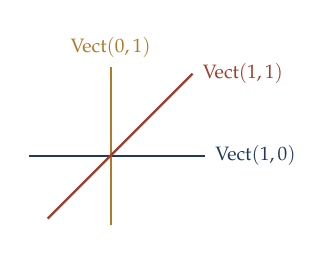
\begin{tikzpicture}[scale=0.8]
  \draw[Bleu,thick] (-1.3,0)--(1.5,0) node[right,font=\scriptsize]{$\vect(1,0)$};
  \draw[Ocre,thick] (0,-1.1)--(0,1.4) node[above,font=\scriptsize]{$\vect(0,1)$};
  \draw[Brique,thick] (-1,-1)--(1.3,1.3) node[right,font=\scriptsize]{$\vect(1,1)$};
\end{tikzpicture}\\[2pt]
\raggedright Intersections deux à deux nulles, mais $(1,0)+(0,1)-(1,1)=0$ : \textbf{pas directe}.
\end{PIEGE}
\end{columns}
\vspace{-4pt}{\small En dimension finie : $E=F\oplus G\iff F\cap G=\{0\}$ \ et \ $\dim F+\dim G=\dim E$.}
\end{frame}

% ---------------------------------------------------------------- EXERCICE 1
\begin{frame}{\badgeexo{1}Un plan et une droite}
\begin{ENONCE}[4 min]
Dans $\R^3$, soit $F$ le plan d'équation $x-y+2z=0$.
\begin{enumerate}
\item Montrer que $G=\vect\big((1,1,1)\big)$ est un supplémentaire de $F$, et décomposer $v=(x,y,z)$ selon $\R^3=F\oplus G$.
\item $H=\vect\big((1,1,0)\big)$ est-il un supplémentaire de $F$ ?
\end{enumerate}
\objectif{la caractérisation par l'intersection et les dimensions.}
\end{ENONCE}
\pause
\begin{INDICE}
Écrire $v=w+m(1,1,1)$ avec $w\in F$, et reporter dans l'équation de $F$.
\end{INDICE}
\end{frame}

\begin{frame}{\badgecor{1}Un plan et une droite}
\begin{columns}[T]
\column{0.4\textwidth}
\begin{RAIS}
Une droite $\vect(u)$ est un supplémentaire d'un plan $F$ de $\R^3$ exactement quand $u\notin F$ : intersection nulle, et $2+1=3$.
\end{RAIS}
\begin{OUTIL}
$E=F\oplus G\iff F\cap G=\{0\}$ et $\dim F+\dim G=\dim E$.
\end{OUTIL}
\column{0.57\textwidth}
\etape{1.} $(1,1,1)$ : $1-1+2=2\neq0$, donc $(1,1,1)\notin F$ : $F\cap G=\{0\}$, et $2+1=3$ : $\R^3=F\oplus G$.\\[3pt]
\pause
Si $v=w+m(1,1,1)$, $w\in F$ : $(x-m)-(y-m)+2(z-m)=0$, donc
\[m=\frac{x-y+2z}2,\qquad v=\underbrace{v-m(1,1,1)}_{\in F}+\underbrace{m(1,1,1)}_{\in G}.\]
\pause
\etape{2.} $1-1+0=0$ : $(1,1,0)\in F$, donc $H\subset F$ : \textbf{non}.
\end{columns}
\end{frame}

\begin{frame}{Projecteurs et symétries}
\begin{columns}[T]
\column{0.5\textwidth}
\begin{DEF}
$E=F\oplus G$, $x=x_F+x_G$ : projection $p(x)=x_F$ sur $F$ parallèlement à $G$ ; symétrie $s(x)=x_F-x_G$ ; \ $s=2p-\Id$.
\end{DEF}
\column{0.46\textwidth}
\begin{PROP}[Caractérisation \livre{prop.~1.6}]
$p\circ p=p$ $\iff$ projecteur, sur $\Im p$ parallèlement à $\Ker p$.\\
$s\circ s=\Id$ $\iff$ symétrie, par rapport à $\Ker(s-\Id)$ parallèlement à $\Ker(s+\Id)$.
\end{PROP}
\end{columns}
\pause
\begin{columns}[T]
\column{0.5\textwidth}
\begin{FORM}[En base adaptée]
$\Mat(p)=\begin{pmatrix}I_r&0\\0&0\end{pmatrix}$, \ $\Mat(s)=\begin{pmatrix}I_r&0\\0&-I_{n-r}\end{pmatrix}$.
\end{FORM}
\column{0.46\textwidth}
\begin{METH}{Calculer $p(x)$}
$G=\vect(w)$ : $t$ tel que $x-tw\in F$ ; $p(x)=x-tw$, $s(x)=x-2tw$.
\end{METH}
\end{columns}
\end{frame}

% =====================================================================
\partie{1.3}{Hyperplans et systèmes}{Comment décrire un sous-espace par des équations ?}{\rmI}

\begin{frame}{Hyperplans}
\begin{DEF}
Hyperplan de $E$ ($\dim E=n$) : sous-espace qui admet une droite comme supplémentaire ; dimension $n-1$.
\end{DEF}
\begin{PROP}[\livre{prop.~1.8}]
\begin{itemize}
\item Hyperplans $=$ noyaux des formes linéaires non nulles : une équation $a_1x_1+\dots+a_nx_n=0$.
\item $H=\Ker\varphi$, $u\notin H$ $\Rightarrow$ $E=H\oplus\vect(u)$ \quad (exercice~1).
\item $p$ hyperplans : intersection de dimension $\geq n-p$ ; un sous-espace de dimension $n-p$ est défini par $p$ équations.
\end{itemize}
\end{PROP}
\begin{EX}[Lecture géométrique]
Dans $\R^3$ : un plan vectoriel $=$ une équation ; une droite $=$ deux équations (deux plans qui se coupent).
\end{EX}
\end{frame}

\begin{frame}{Équations d'un sous-espace, systèmes linéaires}
\begin{METH}{Base $\leftrightarrow$ équations \livre{méth.~1.1}}
\begin{itemize}
\item Équations $\to$ base : résoudre le système.
\item Base $(v_1,\dots,v_k)$ $\to$ équations : $x\in F\iff$ le système $x=\sum\lambda_iv_i$ est compatible ; ses conditions de
compatibilité sont les $n-k$ équations de $F$.
\end{itemize}
\end{METH}
\pause
\begin{columns}[T]
\column{0.5\textwidth}
\begin{EX}
$F=\vect(1,2,3,4)\subset\R^4$ : $y=2x$, $z=3x$, $t=4x$ ; trois hyperplans, $\dim F=4-3$.
\end{EX}
\column{0.46\textwidth}
\begin{RETENIR}
Système homogène de rang $r$ à $n$ inconnues : solutions de dimension $n-r$. Avec second membre : vide, ou $X_0+\Ker A$.
\end{RETENIR}
\end{columns}
\end{frame}

% =====================================================================
\partie{1.4}{Trace}{Un invariant facile à calculer, et ce qu'il interdit.}{\rmI}

\begin{frame}{La trace}
\begin{columns}[T]
\column{0.55\textwidth}
\begin{DEF}
$\tr(A)=\sum_{i=1}^na_{i,i}$ : somme des coefficients diagonaux.
\end{DEF}
\begin{PROP}[\livre{prop.~1.11}]
\begin{itemize}
\item $\tr$ est une forme linéaire : $\Ker\tr$ est un hyperplan ;
\item $\tr(AB)=\tr(BA)$ ;
\item $\tr(P^{-1}AP)=\tr(A)$ : on définit $\tr(f)$.
\end{itemize}
\end{PROP}
\column{0.41\textwidth}
\pause
\textbf{Preuve :}
\[\tr(AB)=\sum_{i,k}a_{i,k}b_{k,i}=\tr(BA).\]
Puis $\tr\big((P^{-1}A)P\big)=\tr\big(P(P^{-1}A)\big)=\tr A$.
\end{columns}
\pause
\begin{columns}[T]
\column{0.48\textwidth}
\begin{EX}[Projecteur]
Base adaptée : $\mathrm{diag}(I_r,0)$, donc $\tr(p)=r=\rg(p)$.
\end{EX}
\column{0.48\textwidth}
\begin{PIEGE}
$\tr(AB)\neq\tr A\,\tr B$ ; \ $\tr(ABC)\neq\tr(BAC)$ en général.
\end{PIEGE}
\end{columns}
\end{frame}

% ---------------------------------------------------------------- EXERCICE 2
\begin{frame}{\badgeexo{2}Semblables ou non ?}
\begin{ENONCE}[5 min]
Les matrices suivantes sont-elles semblables ? Justifier en une ligne.
\[\text{(a)}\ \begin{pmatrix}1&2\\0&3\end{pmatrix}\ \text{et}\ \begin{pmatrix}2&0\\1&2\end{pmatrix}\qquad
\text{(b)}\ I_2\ \text{et}\ \begin{pmatrix}1&1\\0&1\end{pmatrix}\qquad
\text{(c)}\ \begin{pmatrix}1&0\\0&0\end{pmatrix}\ \text{et}\ \begin{pmatrix}0&0\\0&0\end{pmatrix}\]
\objectif{utiliser les invariants, et voir leurs limites.}
\end{ENONCE}
\pause
\begin{INDICE}
Comparer trace, rang et déterminant ($2\times2$, vu en première année). En (b), quelles sont les matrices semblables à $I_2$ ?
\end{INDICE}
\end{frame}

\begin{frame}{\badgecor{2}Semblables ou non ?}
\begin{columns}[T]
\column{0.4\textwidth}
\begin{RAIS}
Un invariant différent suffit pour dire \emph{non}. Mais des invariants égaux ne suffisent pas pour dire \emph{oui}.
\end{RAIS}
\begin{OUTIL}
Rang, trace (et déterminant) invariants par similitude.
\end{OUTIL}
\column{0.57\textwidth}
\etape{(a)} Même trace $4$, mais déterminants $3$ et $4$ : \textbf{non}.\\[4pt]
\pause
\etape{(b)} Même trace $2$, même déterminant $1$, même rang\dots\ mais $P^{-1}I_2P=I_2$ pour toute $P$ : la seule matrice semblable à $I_2$ est $I_2$. \textbf{Non}.\\[4pt]
\pause
\etape{(c)} Rangs $1$ et $0$ : \textbf{non}.
\end{columns}
\begin{ASTU}
(b) prépare le chapitre~3 : $\begin{pmatrix}1&1\\0&1\end{pmatrix}$ ne sera pas diagonalisable.
\end{ASTU}
\end{frame}

% =====================================================================
\partie{1.5}{Sous-espaces stables}{Comment lire sur une matrice qu'un sous-espace est « respecté » par $f$ ?}{\rmI}

\begin{frame}{Sous-espace stable, endomorphisme induit}
\begin{DEF}
$F$ est \emph{stable} par $f$ si $f(F)\subset F$. L'endomorphisme induit $f_F:F\to F$, $x\mapsto f(x)$.
\end{DEF}
\begin{PROP}[\livre{prop.~1.14}]
\begin{itemize}
\item $F=\vect(e_1,\dots,e_p)$ stable $\iff f(e_j)\in F$ pour tout $j$ : on vérifie sur une base.
\item $\Ker f$ et $\Im f$ sont stables par $f$ ; si $f\circ g=g\circ f$, $\Ker g$ et $\Im g$ sont stables par $f$.
\end{itemize}
\end{PROP}
\pause
\textbf{Preuve du second point :} $g(x)=0\Rightarrow g\big(f(x)\big)=f\big(g(x)\big)=0$ ; \ $f\big(g(x)\big)=g\big(f(x)\big)\in\Im g$.
\end{frame}

\begin{frame}{Traduction matricielle : des blocs}
\begin{columns}[c]
\column{0.58\textwidth}
\begin{PROP}[Théorème \livre{th.~1.15}]
Base adaptée à $F$ ($p$ premiers vecteurs dans $F$) :
\[F\text{ stable}\iff\Mat(f)=\begin{pmatrix}A&B\\0&C\end{pmatrix}.\]
$E=F\oplus G$, les deux stables $\iff\begin{pmatrix}A&0\\0&C\end{pmatrix}$.\\
Alors $\tr f=\tr A+\tr C$ (et $\det f=\det A\det C$, chapitre~2).
\end{PROP}
\column{0.38\textwidth}
\centering
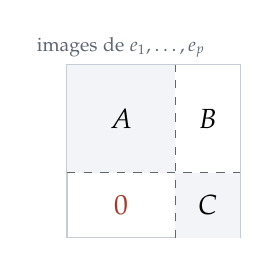
\begin{tikzpicture}[scale=0.55]
  \draw[Filet] (0,0) rectangle (4,4);
  \fill[Fond] (0,1.5) rectangle (2.5,4); \node at (1.25,2.75) {$A$};
  \node at (3.25,2.75) {$B$};
  \node[Brique] at (1.25,0.75) {$0$};
  \fill[Fond] (2.5,0) rectangle (4,1.5); \node at (3.25,0.75) {$C$};
  \draw[Gris,dashed] (2.5,0)--(2.5,4); \draw[Gris,dashed] (0,1.5)--(4,1.5);
  \node[font=\scriptsize,Gris] at (1.25,4.4) {images de $e_1,\dots,e_p$};
\end{tikzpicture}\\[2pt]
{\footnotesize\color{Gris}le $0$ dit : les $f(e_j)$, $j\leq p$, restent dans $F$}
\end{columns}
\pause
\begin{columns}[T]
\column{0.58\textwidth}
\begin{FORM}[Projecteurs, symétries]
$p^2=p$ : $\mathrm{diag}(I_r,0)$ dans $\Im p\oplus\Ker p$.\\
$s^2=\Id$ : $\mathrm{diag}(I_r,-I_{n-r})$ dans $\Ker(s-\Id)\oplus\Ker(s+\Id)$.
\end{FORM}
\column{0.38\textwidth}
\begin{PROP}[Droite stable \livre{prop.~1.16}]
$\vect(u)$ stable $\iff f(u)=\lambda u$.
\end{PROP}
\end{columns}
\end{frame}

% ---------------------------------------------------------------- EXERCICE 3
\begin{frame}{\badgeexo{3}Chercher des droites stables}
\begin{ENONCE}[6 min]
Soit $f$ l'endomorphisme de $\R^3$ de matrice $A=\begin{pmatrix}1&2&0\\2&1&0\\0&0&-1\end{pmatrix}$.
\begin{enumerate}
\item Montrer que le plan $F$ : $z=0$ et la droite $\vect(e_3)$ sont stables par $f$. Que dit la forme de $A$ ?
\item Montrer que les droites engendrées par $(1,1,0)$ et $(1,-1,0)$ sont stables.
\item En déduire une base dans laquelle la matrice de $f$ est diagonale.
\end{enumerate}
\objectif{passer des sous-espaces stables aux vecteurs propres.}
\end{ENONCE}
\end{frame}

\begin{frame}{\badgecor{3}Chercher des droites stables}
\begin{columns}[T]
\column{0.4\textwidth}
\begin{RAIS}
Les blocs se lisent sur $A$ ; une droite est stable quand son vecteur directeur est dilaté. Trois droites stables
supplémentaires : matrice diagonale.
\end{RAIS}
\begin{OUTIL}
Théorème~1.18 ; proposition~1.19.
\end{OUTIL}
\column{0.57\textwidth}
\etape{1.} $f(x,y,0)=(x+2y,2x+y,0)\in F$ ; $f(e_3)=-e_3$. $A$ est diagonale par blocs : $\begin{pmatrix}A_1&0\\0&-1\end{pmatrix}$.\\[3pt]
\pause
\etape{2.} $A(1,1,0)^T=(3,3,0)^T$ : dilatation de rapport $3$. $A(1,-1,0)^T=(-1,1,0)^T$ : rapport $-1$.\\[3pt]
\pause
\etape{3.} $\mathcal B'=\big((1,1,0),(1,-1,0),e_3\big)$ est une base (trois vecteurs non coplanaires), et
\[\Mat_{\mathcal B'}(f)=\mathrm{diag}(3,-1,-1).\]
\end{columns}
\begin{ASTU}
Ces vecteurs, simplement dilatés, sont les \emph{vecteurs propres} : c'est le point de départ du chapitre~3, \emph{Réduction}.
\end{ASTU}
\end{frame}

% =====================================================================
\partie{1.6}{Synthèse}{Devant une question d'algèbre linéaire, par quoi commencer ?}{\rmI}

% ---------------------------------------------------------------- EXERCICE 4
\begin{frame}{\badgeexo{4}Un projecteur donné par sa matrice}
\begin{ENONCE}[6 min]
Soit $u$ l'endomorphisme de $\R^3$ de matrice $A=\dfrac12\begin{pmatrix}1&2&-1\\0&2&0\\-1&2&1\end{pmatrix}$.
\begin{enumerate}
\item Vérifier que $A^2=A$. Que vaut $\rg u$ sans calcul ?
\item Donner une base de $\Ker u$ et de $\Im u$, puis une base où la matrice de $u$ est $\mathrm{diag}(0,1,1)$.
\end{enumerate}
\objectif{reconnaître un projecteur et utiliser la base adaptée.}
\end{ENONCE}
\pause
\begin{INDICE}
Pour un projecteur, rang $=$ trace, et $E=\Ker u\oplus\Im u$.
\end{INDICE}
\end{frame}

\begin{frame}{\badgecor{4}Un projecteur donné par sa matrice}
\begin{columns}[T]
\column{0.4\textwidth}
\begin{RAIS}
$A^2=A$ : $u$ est la projection sur $\Im u$ parallèlement à $\Ker u$ ; il suffit d'une base de chacun.
\end{RAIS}
\begin{OUTIL}
Proposition~1.9 ; $\tr p=\rg p$.
\end{OUTIL}
\column{0.57\textwidth}
\etape{1.} Le calcul donne $A^2=A$ : projecteur, et $\rg u=\tr A=\frac12+1+\frac12=2$.\\[3pt]
\pause
\etape{2.} $\Ker u$ : $y=0$ et $x=z$, soit $\vect(1,0,1)$. $\Im u$ : engendrée par les colonnes, base $\big((1,0,-1),(1,1,1)\big)$
(équation $x-2y+z=0$).\\[3pt]
\pause
Dans la base $\big((1,0,1),(1,0,-1),(1,1,1)\big)$, adaptée à $\Ker u\oplus\Im u$ : $\mathrm{diag}(0,1,1)$.
\end{columns}
\end{frame}

\begin{frame}{Quelle méthode ?}
\small
\renewcommand{\arraystretch}{1.28}
\begin{tabular}{@{}p{4.6cm}p{9.2cm}@{}}
\toprule
\textbf{Question} & \textbf{Méthode}\\\midrule
$\rg u$, $\dim\Ker u$ ? & base de l'image, puis théorème du rang\\
$E=F\oplus G$ ? & intersection nulle et somme des dimensions\\
projecteur, symétrie ? & $f\circ f=f$, $f\circ f=\Id$ ; base adaptée\\
calculer une projection & $x-tw\in F$ donne la composante sur $G=\vect(w)$\\
équations d'un sous-espace & conditions de compatibilité de $x=\sum\lambda_iv_i$\\
trace & linéaire ; $\tr(AB)=\tr(BA)$ ; $\tr p=\rg p$\\
$F$ stable par $f$ ? & images d'une base de $F$ ; forme triangulaire par blocs\\\bottomrule
\end{tabular}
\end{frame}

\begin{frame}{Pièges et essentiel}
\begin{columns}[T]
\column{0.48\textwidth}
\begin{PIEGE}[Pièges fréquents]
\begin{itemize}
\item Somme directe de trois sous-espaces : les intersections deux à deux ne suffisent pas.
\item $E=F\oplus G$ : il faut aussi la somme, ou les dimensions.
\item Matrice de passage : nouveaux vecteurs dans l'ancienne base ; $P^{-1}AP$.
\item $\Ker f$ et $\Im f$ pas toujours supplémentaires.
\item $\tr(AB)\neq\tr A\tr B$.
\end{itemize}
\end{PIEGE}
\column{0.48\textwidth}
\begin{RETENIR}
\begin{itemize}
\item Théorème du rang ; semblables : même rang, même trace.
\item Somme directe $\iff$ unicité de la décomposition de $0$.
\item $p^2=p$, $s^2=\Id$ ; bases adaptées.
\item Hyperplan $=\Ker\varphi$, $\varphi\neq0$ ; $p$ équations : $\dim\geq n-p$.
\item Stable $\iff$ blocs ; droite stable $\iff f(u)=\lambda u$.
\end{itemize}
\end{RETENIR}
\end{columns}
\end{frame}

\begin{frame}{Après la séance}
\begin{columns}[T]
\column{0.52\textwidth}
\begin{enumerate}
\item \textbf{Relire le livret} (chapitre~1) : démonstrations et exemples rédigés.
\item \textbf{Apprendre la fiche}, puis faire l'\textbf{exercice bilan} (15 min).
\item \textbf{Cinq problèmes} de la sélection, dans l'ordre :
\begin{itemize}\small
\item deux plans supplémentaires de $\R^4$ ;
\item les polynômes de Lagrange ;
\item la trace et les commutateurs ;
\item les endomorphismes de carré nul ;
\item somme de deux projecteurs.
\end{itemize}
\item Puis le \textbf{TD complet} (22 exercices, quatre niveaux).
\end{enumerate}
\column{0.42\textwidth}
\begin{ASTU}[Pour chercher seul]
Lire l'en-tête du problème, chercher au brouillon, ne lire qu'\emph{une} indication en cas de blocage, la correction à la fin.
\end{ASTU}
\begin{ASTU}[La suite]
Chapitre~2, \emph{Déterminants}, puis chapitre~3, \emph{Réduction} : les droites stables deviennent des vecteurs propres.
\end{ASTU}
\end{columns}
\end{frame}

\end{document}
